
\newpage
\section{Einführung (ca. 4 Seiten/2.5)}
\label{Einführung}
\subsection{Motivation}
\iffalse
Erkläre, warum das Thema Media \ac{ROAS} im Kontext von bonprix relevant ist.
Diskutiere die Bedeutung von Marketing-Analysen in der heutigen digitalen Welt und wie sie Unternehmen helfen, ihre Strategien zu optimieren.
Füge aktuelle Statistiken oder Beispiele aus der Branche hinzu, um deine Argumente zu untermauern.
\fi
\subsection{Zielsetzung der Arbeit}
\label{ZielsetzungDerArbeit}
Das Ziel dieser Arbeit ist es, die Effizienz verschiedener Media-Kanäle zu analysieren, um eine optimale Verteilung der Werbeausgaben zu realisieren. \\
Die folgenden Fragen sollen in dieser Arbeit beantwortet werden:
\begin{itemize}
    \item Wie verhalten sich die Mediaausgaben und sind die Daten in Bezug zu der Nachfrageänderung nachvollziehbar? 
    \item Wie sieht die Verteilung der Nachfrageeffekte der Unterkanäle in Media aus?
    \item  Wie ist der ROAS der verschiedenen Unterkanäle in Media?
    \item Sind die Ergebnisse des Marketing-Mix-Modells nachvollziehbar? 
\end{itemize} 
Die erste Frage ist herausfordernd, da Mediaausgaben in der Regel in Kampagnen getätigt werden. Das heißt, dass die Mehrheit der Tage die Mediaausgaben einen Nullwert aufweisen. Nur zu den Kampagnenzeiten weist diese Zeitreihe Ausgaben auf.\\
Im Rahmen der Bachelorarbeit werden die folgenden methodischen Schritte umgesetzt:
\begin{enumerate}
    \item Die Methoden werden in die Arbeit eingearbeitet. Sowohl die lineare als auch die multiple lineare Regression, die Methode der kleinsten Quadrate und die Huber-Loss-Funktion werden definiert. Ihre Funktionsweisen werden ausführlich behandelt.
    \item Eine deskriptive Analyse wird auf verarbeitete Daten durchgeführt, um die Mediaausgaben zu untersuchen. Dabei wird auch auf die Nachvollziehbarkeit der Daten, beispielsweise die Verteilung der Mediaausgaben, eingegangen.
    \item Anwendung der Wavelet-Funktion, um die für Media relevante Nachfrage herauszufiltern.
    \item Eine Huber-Regression wird auf die gefilterten Nachfragedaten angewandt.
    \item Gegebenenfalls der Fachabteilung das Ergebnis zeigen, um die Nachvollziehbarkeit und Richtigkeit zu prüfen.
\end{enumerate}
Dabei könnte Schritt vier durch einen Austausch in der Datenwissenschaftsabteilung ersetzt werden, wenn die Kapazitäten eng werden.   
\subsection{Aufbau der Arbeit}
Die vorliegende Bachelorarbeit ist in fünf Kapitel unterteilt, die einen systematischen Überblick über die Forschung zu \ac{MMM} und die Integration der Huber-Loss-Funktion geben.\\\\
Das erste Kapitel \nameref{Einführung} führt in die grundlegende Problemstellung ein und betont die Relevanz der Problemlösung für den Betrieb. In diesem Kapitel werden die Forschungsfragen aufgelistet und erklärt. Es wird beschrieben, was in dieser Arbeit erreicht wird und wie das Ziel zu erreichen ist. \\\\
Das zweite Kapitel \nameref{GeschäftlicheGrundlagen} beschreibt die Grundlagen des \ac{MMM} und definiert Media-Kanäle. Es wird auch beschrieben, welche Erfahrungen andere Unternehmen zur Kostenaufteilung in Media-Kanäle haben. Zum Schluss wird der aktuelle Zustand des \ac{MMM}s bei bonprix beschrieben, und die Media-Kanäle bei bonprix werden vorgestellt. \\\\ 
Im dritten Kapitel \nameref{TheoretischeGrundlagen} wird die Methodik des Vorgehens beschrieben. Es wird erläutert, was eine deskriptive Analyse ist und wie die lineare sowie die multiple lineare Regression funktionieren. Anschließend werden die statistischen Grundlagen wie die Methode der kleinsten Quadrate und die Huber-Loss-Funktion vorgestellt.\\\\
Das vierte Kapitel \nameref{Umsetzung} dokumentiert die Arbeitsschritte. Es fängt mit einer Vorstellung der Daten an. Die Daten werden verarbeitet für den Einsatz und die deskriptive Analyse wird eingesetzt. In der deskriptiven Analyse wird der Verlauf der Mediaausgaben und Nachfrage untersucht und die Aufteilung der Mediaausgaben wird visualisiert.  
\iffalse
bonprix Handelsgesellschaft mbH hat ein Marketing-Mix-Modell. Marketing-Mix-Modell quantifiziert die Effekte verschiedener Marketingtaktiken basierend auf der Nachfrage \cite{MMMdef}. Das Marketing-Mix-Modell bei bonprix umfasst die internen Faktoren, die externen Faktoren, Wettbewerber und Marketingkanäle. Media, als ein Teil von Marketingkanälen, enthält TV, Radio, Out Of Home (Engl. Außer Haus) etc. Unter Out Of Home sind alle Werbemedien im öffentlichen Raum, wie Plakate, zu verstehen. \\\\
Das Marketing-Mix-Modell differenziert nicht mehr zwischen den einzelnen Unterkanälen im Medienbereich. Wenn bonprix einen bestimmten Betrag für Medieninvestitionen ausgibt, fehlt eine Orientierung zu den Nachfrageeffekten der Unterkanäle und zur optimalen Kostenaufteilung.

bonprix zahlt einen bestimmten Betrag für das Marketing. \\ 
Es gibt 3 oberkategorien: Media, Katalog, Online-Marketing. wie viel marketing, media tv radio youtube, wenn 100mio wie viel gibt man wo aus, da am meisten investieren wo mehr nachfragen sind, 

Regressionsansatz, simple statistische regression, wie viele nachfragte durch media katalog und oma... VF aber hohe kosten, saisonalität sommer mehr und winter weniger, märz bis juli mehr nachfrage, linearer trend konjunktor, wettbewerber wenn andere mehr zahlen dann wir weniger, erklärende variablen bubbles draussen, nltrend nicht linearer trend, betas sind gewichte, beta bestimmt einfluss von einzelnen punkten, bspl oma 2,5, a ist grundnachfrage ohne alles, et ist das was man nicht erklären kann also error, saison nicht nur sommer winter in der woche auch zum beispiel WE mehr nachfrage, t ist index für Tag,
Methodik: Regression, nachfrage zerlegen in oma media...deskriptive analyse zuerst als plots, verhältnis, korrelation, parallel analysieren und schreiben, circle: daten auswahl, analyse, knowledge discovering in databases, \\ \\
Problematik: Unter Media unklar, welcher Kanal mehr Nachfrage generiert. Kosten Media = Kosten tv + Kosten ooh + Kosten radio + Youtube + Digital Media (ich weiß nicht ganz genau aber sind auch Videos online glaub ich) + OLV (Online Video) etc.
Das soll aufgesplittet werden, sodass im Modell wir jeweils einen Effekt für TV, OOH, Radio etc. haben
Ziel: media ohne Katalog? entweder ohne katalog oder bestimmte zeitrahmen aber am ende klären.  
ein mal im monat katalog schicken daher ein peak,

logit
probit
poisson
xgboosted
lasso

warum nicht früher gesplittet?

media und OMA müssen besser getrennt sein
nachfrage formel ob eher multiplikation statt plus? Moderationseffekte (=Interaktionseffekte), wenn alle Faktoren zusammenspielen/interagieren, führt es zum kauf.
mediationseffekte: ein faktor wirkt indirekt, zb Wochenende, saisonal... meistens Markenverfügbarkeit indirekt-> Nachfrage -> Markenbekanntheit, 
multiple source effect 
wie ist die nachfrage skaliert, definiert? Wie ist die Nachfrage verteilt?
histogramm: y-achse häufigkeit, x-achse ausprägungen der variablen: euro, prozent, skala wie 10/10...wann ist nachfrage gering, hoch normal...

Titel herausfinden

wavelet auch schreiben oder überspringen?


\begin{figure} [h]
    \centering
    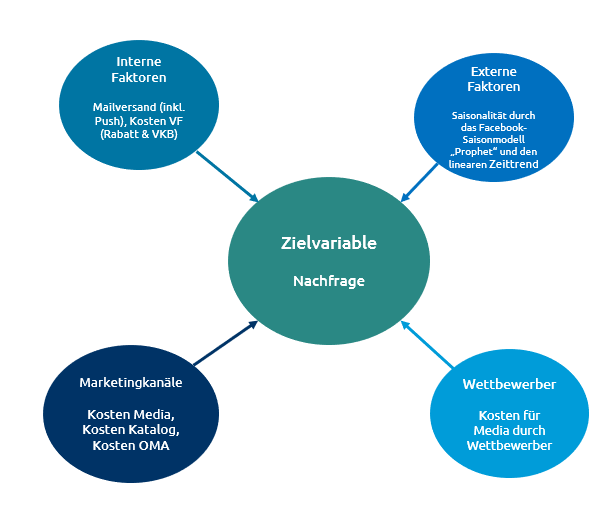
\includegraphics[width=0.75\linewidth]{mmm.png}
    \caption{\ac{MMM}-Modell bei bonprix}
    \label{fig:mmm-label}
\end{figure}


Kommentar 
\fi
